% SC4023 --- Chapter 1: Introduction: AI Meets Software Engineering (0->100 ground-up)
\chapter{Introduction: Where AI Meets Software Engineering}
\label{ch:intro-ai4se}
\sloppy

\begin{quote}
\emph{``Programs must be written for people to read, and only incidentally for machines to execute.''} --- Harold Abelson. When programs grew from hundreds to millions of lines, reading, writing, and fixing them became a human bottleneck. AI now offers to read, write, and fix alongside us.
\end{quote}

\noindent\fbox{\parbox{\dimexpr\linewidth-2\fboxsep-2\fboxrule}{%
\textbf{From zero: no AI or SE background assumed.} We build from everyday intuition---what it means to build reliable software, why it is hard, and where a learning machine can help---before any model or metric. Every term is defined on first use, picture first, then formalism. This chapter is the map for the whole book.}}
\vspace{0.4em}

\section*{Learning Outcomes}
After this chapter you will be able to:
\begin{enumerate}[label=(L\arabic*)]
    \item describe the software engineering lifecycle and name its core phases and artefacts;
    \item explain why scale, complexity, and human factors make SE hard and costly;
    \item classify AI-for-SE tasks (generation, testing, repair, requirements, management);
    \item distinguish the direction AI$\to$SE from SE$\to$AI and give examples of each;
    \item state the key challenges---data quality, evaluation, and trust---that bound what AI can do.
\end{enumerate}

% ============================================================
\section{What Is Software Engineering?}
\label{sec:what-is-se}
\paragraph{Intuition.} Imagine building a bridge. You do not start by welding steel; you survey the river, sketch designs, estimate load, pour foundations, test every joint, and schedule inspections for decades. Software is similar, but the bridge is invisible, changes weekly, and must carry millions of users at once. \emph{Software engineering} (SE) is the disciplined process for building that invisible bridge so it does not collapse under its own weight.

\paragraph{Formal view.} The \emph{software development lifecycle} (SDLC) organises work into phases: \emph{requirements} (what to build), \emph{design} (how to structure it), \emph{implementation} (writing code), \emph{verification} (testing and review), and \emph{maintenance} (fixing and evolving). Each phase produces \emph{artefacts}: specifications, architecture diagrams, source code, test suites, and issue reports. A \emph{process model} (waterfall, agile, DevOps) orders and iterates these phases.

\begin{definition}[Software engineering]
\emph{Software engineering} is the systematic application of engineering principles---abstraction, decomposition, measurement, and process---to the design, construction, verification, and evolution of software systems under constraints of time, cost, and quality.
\end{definition}

\begin{figure}[h]\centering
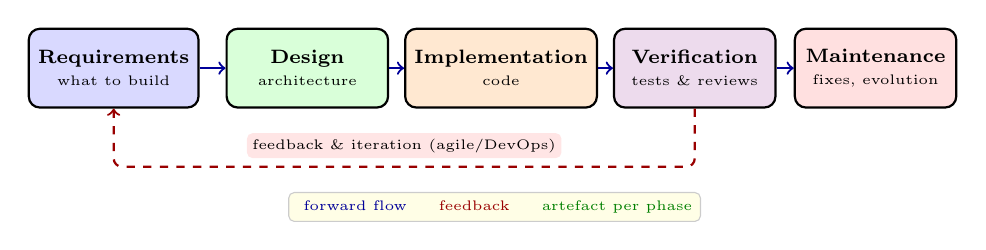
\begin{tikzpicture}[scale=0.82,every node/.style={font=\scriptsize},
  phase/.style={draw, thick, rounded corners=4pt, minimum width=2.05cm, minimum height=1.0cm, align=center}]
  \node[phase, fill=blue!15] (req) at (0,0) {\textbf{Requirements}\\\tiny what to build};
  \node[phase, fill=green!15] (des) at (3.0,0) {\textbf{Design}\\\tiny architecture};
  \node[phase, fill=orange!18] (imp) at (6.0,0) {\textbf{Implementation}\\\tiny code};
  \node[phase, fill=violet!14] (ver) at (9.0,0) {\textbf{Verification}\\\tiny tests \& reviews};
  \node[phase, fill=red!12] (mnt) at (11.8,0) {\textbf{Maintenance}\\\tiny fixes, evolution};
  \foreach \a/\b in {req/des,des/imp,imp/ver,ver/mnt}
    \draw[->,thick,blue!60!black] (\a) -- (\b);
  \draw[->,thick,red!60!black,dashed,rounded corners=3pt] (ver.south) -- ++(0,-0.9) -- ++(-9,0) -- (req.south);
  \node[font=\tiny,fill=red!10,rounded corners=2pt,inner sep=2pt] at (4.5,-1.2) {feedback \& iteration (agile/DevOps)};
  \node[font=\tiny,align=left,fill=yellow!10,draw=gray!40,rounded corners=2pt,inner sep=3pt] at (5.9,-2.15) {\textcolor{blue!60!black}{$\blacksquare$ forward flow} \quad \textcolor{red!60!black}{$\blacksquare$ feedback} \quad \textcolor{green!50!black}{$\blacksquare$ artefact per phase}};
\end{tikzpicture}
\caption{The SE lifecycle as a pipeline with feedback. Each box produces an artefact; arrows are hand-offs. Modern processes iterate rapidly around this loop rather than traversing it once.}
\label{fig:se-pipeline}
\end{figure}

Each hand-off is a translation: natural-language needs become specifications, specifications become code, code becomes behaviour checked by tests. Every translation can introduce defects, and defects become exponentially costlier when discovered late. That cost curve is the economic reason SE needs help.

An old debate contrasts \emph{plan-driven} (waterfall: freeze requirements, then design and build) with \emph{iterative} (agile/DevOps: short sprints, continuous feedback). In practice, both produce the same artefacts; they differ in batch size and how quickly feedback loops close. AI assistance is valuable in either model because it shortens each translation and tightens each loop.

% ============================================================
\section{Why Software Engineering Needs AI}
\label{sec:why-ai}
\paragraph{Intuition.} A single developer can hold a few thousand lines in mind. A modern product holds tens of millions, changes hundreds of times per day, and is touched by hundreds of contributors across time zones. No human can see the whole system at once, yet every change can break it. AI helps because much of SE work is \emph{patterned}: similar bugs recur, similar tests are needed, similar code is written again and again.

Three forces create the need. First, \emph{scale}: codebases, logs, and issue trackers generate far more data than any team can read. Second, \emph{complexity}: interactions between components are combinatorial and non-local; a one-line change can fail a distant test. Third, \emph{human limits}: fatigue, context switching, and incomplete knowledge cause mistakes. AI, trained on millions of prior examples, can surface relevant patterns fast, draft candidates, and flag risks---not replacing judgement but amplifying it.

\begin{figure}[h]\centering
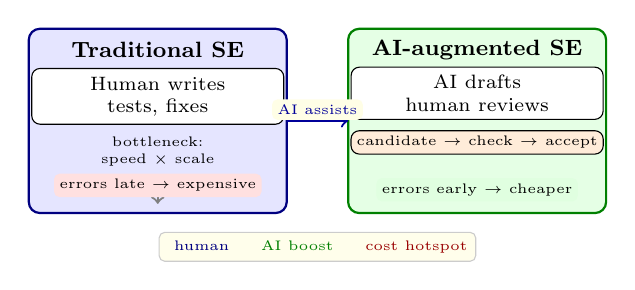
\begin{tikzpicture}[scale=0.78,every node/.style={font=\scriptsize}]
  \draw[fill=blue!10,draw=blue!50!black,thick,rounded corners=4pt] (0,0) rectangle (4.2,3.0);
  \node[font=\footnotesize\bfseries] at (2.1,2.65) {Traditional SE};
  \node[draw,fill=white,rounded corners=3pt,minimum width=3.2cm,align=center,inner sep=3pt] at (2.1,1.9) {Human writes\\tests, fixes};
  \node[font=\tiny,align=center] at (2.1,1.0) {bottleneck:\\speed $\times$ scale};
  \draw[->,thick,gray] (2.1,0.55) -- (2.1,0.15);
  \node[font=\tiny,fill=red!12,rounded corners=2pt,inner sep=2pt] at (2.1,0.45) {errors late $\to$ expensive};
  \draw[fill=green!10,draw=green!50!black,thick,rounded corners=4pt] (5.2,0) rectangle (9.4,3.0);
  \node[font=\footnotesize\bfseries] at (7.3,2.65) {AI-augmented SE};
  \node[draw,fill=white,rounded corners=3pt,minimum width=3.2cm,align=center,inner sep=3pt] at (7.3,1.95) {AI drafts\\human reviews};
  \node[draw,fill=orange!15,rounded corners=3pt,inner sep=2pt,font=\tiny] at (7.3,1.15) {candidate $\to$ check $\to$ accept};
  \node[font=\tiny,fill=green!12,rounded corners=2pt,inner sep=2pt] at (7.3,0.38) {errors early $\to$ cheaper};
  \draw[->,thick,blue!60!black] (4.2,1.5) -- (5.2,1.5) node[midway,above,font=\tiny,fill=yellow!10,rounded corners=2pt,inner sep=2pt] {AI assists};
  \node[font=\tiny,align=left,fill=yellow!8,draw=gray!40,rounded corners=2pt,inner sep=3pt] at (4.7,-0.55) {\textcolor{blue!50!black}{$\blacksquare$ human} \quad \textcolor{green!50!black}{$\blacksquare$ AI boost} \quad \textcolor{red!60!black}{$\blacksquare$ cost hotspot}};
\end{tikzpicture}
\caption{Why AI helps: the traditional bottleneck shifts when AI drafts and humans review, catching defects earlier where fixes are cheapest.}
\label{fig:why-ai}
\end{figure}

\begin{example}[The cost-of-delay curve]
Boehm's classic data shows a defect found in requirements costs $1\times$ to fix, in design $5\times$, in coding $10\times$, in testing $50\times$, and in production $100$--$1000\times$. Any tool that moves detection one phase earlier pays for itself, even if it is imperfect. AI code review that catches a null dereference at write-time saves the production incident that would have followed.
\end{example}

A complementary view is \emph{cognitive load}: developers spend roughly 60\% of time comprehending code, not writing it. Tools that summarise, navigate, or explain code reduce that load directly, even when they do not generate a single line.

\paragraph{A concrete slice: from issue to patch.} Consider a real loop: a user files issue ``app crashes when name is empty,'' a developer reproduces it, localises the null dereference, writes a guard, adds a test, and opens a pull request. Each step involves reading artefacts (issue text, stack trace, surrounding code), deciding, and writing. An AI assistant can help at every step: summarise the issue, suggest the suspicious lines, draft the guard and the test, and explain the change in the PR description. The human still decides, but the loop is shorter.

\begin{definition}[SE artefact]
An \emph{artefact} is any persistent product of the lifecycle: a requirement sentence, a design diagram, a source file, a test case, a bug report, or a log trace. AI-for-SE treats artefacts as data: it learns joint distributions over them and predicts missing or next artefacts given observed ones.
\end{definition}

% ============================================================
\section{A Taxonomy of AI for SE}
\label{sec:taxonomy}
\paragraph{Intuition.} Not all AI help looks the same. Sometimes AI \emph{writes} (code, tests, docs); sometimes it \emph{checks} (finds bugs, predicts risk); sometimes it \emph{decides} (prioritises issues, assigns reviewers). A simple map prevents confusion about what is being automated and how to evaluate it.

We organise AI-for-SE along two axes: \emph{artefact} (requirements, code, tests, defects, process) and \emph{role} (generate, analyse, predict, assist). This yields five active fronts: \emph{code generation} (Ch.~2), \emph{test generation} (Ch.~3), \emph{program repair} (Ch.~4), \emph{requirements and comprehension}, and \emph{management and prediction} (effort, review, triage). A sixth, \emph{SE for AI}, flips the direction---how SE practices make AI systems reliable, tested, and maintainable.

\begin{figure}[h]\centering
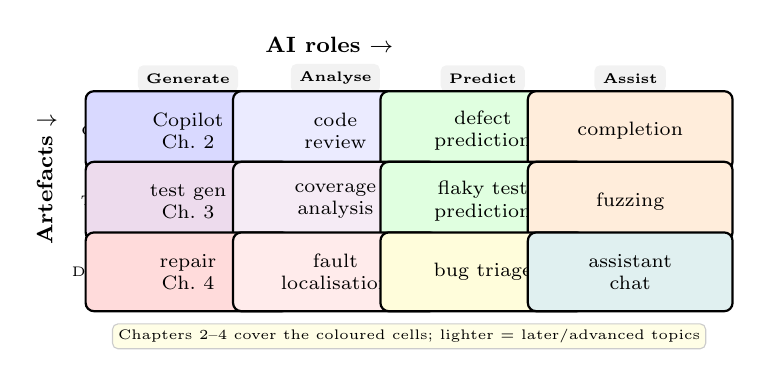
\begin{tikzpicture}[scale=0.78,every node/.style={font=\scriptsize},
  cell/.style={draw,thick,rounded corners=3pt,minimum width=2.6cm,minimum height=1.0cm,align=center}]
  \node[font=\footnotesize\bfseries] at (3.9,4.4) {AI roles $\to$};
  \node[font=\footnotesize\bfseries,rotate=90] at (-0.7,2.2) {Artefacts $\downarrow$};
  \foreach \x/\txt in {1.6/Generate,4.0/Analyse,6.4/Predict,8.8/Assist}
    \node[font=\tiny\bfseries,fill=gray!10,rounded corners=2pt,inner sep=3pt] at (\x,3.85) {\txt};
  \node[font=\tiny,align=right] at (0.2,3.0) {Code};
  \node[cell,fill=blue!15] at (1.6,3.0) {Copilot\\Ch.~2};
  \node[cell,fill=blue!8] at (4.0,3.0) {code\\review};
  \node[cell,fill=green!12] at (6.4,3.0) {defect\\prediction};
  \node[cell,fill=orange!14] at (8.8,3.0) {completion};
  \node[font=\tiny,align=right] at (0.2,1.85) {Tests};
  \node[cell,fill=violet!14] at (1.6,1.85) {test gen\\Ch.~3};
  \node[cell,fill=violet!8] at (4.0,1.85) {coverage\\analysis};
  \node[cell,fill=green!12] at (6.4,1.85) {flaky test\\prediction};
  \node[cell,fill=orange!14] at (8.8,1.85) {fuzzing};
  \node[font=\tiny,align=right] at (0.2,0.70) {Defects};
  \node[cell,fill=red!14] at (1.6,0.70) {repair\\Ch.~4};
  \node[cell,fill=red!8] at (4.0,0.70) {fault\\localisation};
  \node[cell,fill=yellow!14] at (6.4,0.70) {bug triage};
  \node[cell,fill=teal!12] at (8.8,0.70) {assistant\\chat};
  \node[font=\tiny,fill=yellow!10,rounded corners=2pt,inner sep=2pt,draw=gray!40] at (5.2,-0.35) {Chapters~2--4 cover the coloured cells; lighter = later/advanced topics};
\end{tikzpicture}
\caption{Taxonomy of AI-for-SE. Rows are artefacts, columns are roles. Colour groups related tasks; this book focuses on the three most mature code-adjacent cells.}
\label{fig:ai4se-taxonomy}
\end{figure}

\begin{lstlisting}[language=Python, caption={Mining a tiny SE signal: does churn predict defects? A toy illustration of the data AI learns from.}, label={lst:churn-defect}]
# Each commit: lines changed (churn) and whether it introduced a bug (0/1)
commits = [(120,0),(800,1),(45,0),(600,1),(300,0),(950,1),(20,0)]
threshold = 500  # simple rule: high churn -> flag for review
for churn, bug in commits:
    flag = "REVIEW" if churn > threshold else "ok"
    print(f"churn={churn:3d}  bug={bug}  -> {flag}")
# Real models use dozens of features (author, files, time, history).
# The point: SE artefacts are data; patterns in them are learnable.
\end{lstlisting}

The same data view applies everywhere: requirements need ambiguity detection, code needs completion, tests need generation, and issues need triage. Different models (LLMs, classifiers, search) fit different cells, but the workflow is shared---learn from history, propose, let humans decide.

\begin{lstlisting}[language=Python, caption={From pattern to assistant: the AI-for-SE loop in miniature.}, label={lst:ai4se-loop}]
def ai_for_se_loop(history, new_task):
    """History = list of (artefact, outcome). New task = current artefact."""
    patterns = learn_patterns(history)      # e.g., frequent bug patterns
    candidates = generate(patterns, new_task)  # draft code/tests/fixes
    ranked = rank_by_confidence(candidates)    # model scores
    # Human in the loop: review, test, accept or reject
    return [c for c in ranked if human_review(c)]

def learn_patterns(history): return {"null-check": 0.9, "off-by-one": 0.7}
def generate(patterns, task): return [f"candidate for {task} via {p}" for p in patterns]
def rank_by_confidence(cs): return sorted(cs, reverse=True)
def human_review(c): return True  # stub: real review runs tests + inspection
\end{lstlisting}

% ============================================================
\section{Two Directions: AI for SE and SE for AI}
\label{sec:two-directions}
\paragraph{Intuition.} There are two streets between AI and SE, and they carry traffic in opposite directions. \emph{AI for SE} uses learning to help build software (the focus of this book). \emph{SE for AI} uses engineering discipline to make AI systems themselves reliable. Confusing the two leads to mismatched expectations---a great code generator still needs versioning, testing, and monitoring like any other component.

Examples clarify. AI-for-SE: Copilot completes a function, a classifier predicts which commit will be buggy, a repair bot drafts a patch. SE-for-AI: data versioning for training sets, model regression tests that fail when accuracy drops, canary deployments for an LLM service, and experiment tracking that reproduces a model from six months ago. The latter is not optional: without it, ``it worked on my notebook'' becomes the new ``it worked on my machine.''

\begin{definition}[AI for SE vs.\ SE for AI]
\emph{AI for SE} applies AI techniques to SE tasks (code, test, repair, review). \emph{SE for AI} applies SE techniques to AI systems (data pipelines, model testing, deployment, monitoring, and governance). Modern products need both, but this textbook emphasises the first while noting where the second is required.
\end{definition}

A simple check: if the artefact being produced is traditional software (a feature, a test, a fix), you are doing AI-for-SE; if the artefact is a model, dataset, or inference service that must itself be engineered, you are doing SE-for-AI. Teams that master both ship faster and break less.

% ============================================================
\section{Challenges, Limits, and How to Read This Book}
\label{sec:challenges}
What AI cannot do matters as much as what it can. Three limits recur. \emph{Data quality}: training on public code inherits bugs, secrets, and biases; garbage in, garbage out. Duplicated or leaked test data inflates benchmark scores while hiding real weaknesses. \emph{Evaluation}: passing a benchmark (e.g., HumanEval) does not mean the tool helps on your codebase, with your tests, under your deadlines. Lab metrics and field utility diverge. \emph{Trust and accountability}: generated code must be reviewed, tested, and owned; an accepted suggestion is still the developer's responsibility. Ethical and legal questions---licensing of training data, leakage of credentials, over-reliance, and deskilling---sit on top of technical ones.

A practical mental model is \emph{assistant, not autopilot}: AI proposes, humans dispose. Every chapter therefore pairs a generation capability with its checking counterpart---how to test generated code (Ch.~3), how to validate a repair (Ch.~4), and how to measure whether the help actually helped (productivity, quality, and risk metrics introduced next). The field moves fast, but the checking principles---specifications, tests, and careful measurement---are durable.

\paragraph{How to use this book.} Each chapter follows intuition $\to$ formal definition $\to$ worked example $\to$ proof or analysis $\to$ exercises. Chapters~2--4 are the technical core (generation, testing, repair) and can be read independently after this introduction, though they share vocabulary introduced here. Exercises include both conceptual checks and small hands-on prompts you can run with any public LLM or IDE assistant. When you try a prompt, record what you gave, what you got, and how you checked it---that habit is the core skill the book teaches.

% ============================================================
\section{Chapter Notes}
Further reading: Pressman and Maxim's \emph{Software Engineering: A Practitioner's Approach} for the lifecycle; Boehm (1981) for the cost-of-change curve; Harman et~al.\ (2015) for the vision of AI-for-SE; recent surveys by Watson et~al.\ (2022) and Fan et~al.\ (2023) for the generation/testing/repair landscape. Historical note: the term ``software engineering'' was coined at the 1968 NATO conference to argue that building software needed the discipline of other engineering fields---the same argument now motivates AI assistance.

\begin{remark}[Reading tip]
When you encounter an AI-SE claim (e.g., ``tool X improves productivity by 55\%''), ask three questions: What was the task? What was the baseline? What was the measure? The same tool can look brilliant on completion benchmarks and modest on bug-fix rates. Chapters~2--4 train you to ask those questions for generation, testing, and repair respectively.
\end{remark}

A note on terminology: we use \emph{AI}, \emph{ML}, and \emph{LLM} loosely in this introduction. Later chapters are precise: Ch.~2 distinguishes language models from code models and prompting from fine-tuning; Ch.~3 distinguishes search-based from learning-based test generation; Ch.~4 distinguishes heuristic repair from learned repair.

% ============================================================
\section{Exercises}
\label{sec:ch01-exercises}
\begin{enumerate}[label=E1.\arabic*, leftmargin=*, itemsep=0.7em]
    \item \textbf{Lifecycle mapping.} Pick a familiar app (e.g., a campus food-ordering app). List one concrete artefact for each SDLC phase and one feedback arrow from Fig.~\ref{fig:se-pipeline} that would fire when a late requirement changes. Explain why the feedback costs more than catching it early.
    \item \textbf{Cost curve.} A defect costs \$100 if found in requirements, \$500 in design, \$1{,}000 in coding, \$5{,}000 in testing, and \$50{,}000 in production. A team finds 20 defects, evenly spread across phases. Compute total cost. If an AI review tool moves half the production defects to coding, what is the saving?
    \item \textbf{Taxonomy placement.} For each task, place it in Fig.~\ref{fig:ai4se-taxonomy}: (a) summarising a pull request, (b) predicting which files are most likely to contain bugs next release, (c) generating JUnit tests from a method signature, (d) auto-fixing a null-pointer crash. State the row and column and justify in one sentence.
    \item \textbf{AI$\to$SE vs.\ SE$\to$AI.} Give one example of AI helping SE and one of SE helping AI. For the second, explain which SE practice (testing, versioning, or monitoring) matters most for a deployed LLM service and why retraining alone is insufficient.
    \item \textbf{Trust and evaluation.} A code-generation model scores 75\% on HumanEval but your team observes only 30\% of its suggestions are accepted. Propose two distinct hypotheses for the gap and design a one-week A/B experiment on your repository that would distinguish them.
\end{enumerate}
% End of Chapter 1
